\documentclass[11pt]{article}
\usepackage[utf8]{inputenc} % Para caracteres en espa�ol
\usepackage{amsmath,amsthm,amsfonts,amssymb,amscd}
\usepackage{multirow,booktabs}
\usepackage[table]{xcolor}
\usepackage{fullpage}
\usepackage{lastpage}
\usepackage{enumitem}
\usepackage{multicol}
\usepackage{fancyhdr}
\usepackage{mathrsfs}
\usepackage{wrapfig}
\usepackage{setspace}
\usepackage{esvect}
\usepackage{calc}
\usepackage{multicol}
\usepackage{cancel}
\usepackage{graphicx}
\graphicspath{ {pictures/} }
\usepackage[retainorgcmds]{IEEEtrantools}
\usepackage[margin=3cm]{geometry}
\usepackage{amsmath}
\newlength{\tabcont}
\setlength{\parindent}{0.0in}
\setlength{\parskip}{0.05in}
\usepackage{empheq}
\usepackage{framed}
\usepackage{newtxmath}
\usepackage{euscript}
\DeclareMathAlphabet{\mathpzc}{T1}{pzc}{m}{it}
\usepackage[most]{tcolorbox}
\usepackage{xcolor}
\colorlet{shadecolor}{orange!15}
\parindent 0in
\parskip 12pt
\geometry{margin=1in, headsep=0.25in}
\theoremstyle{definition}
\newtheorem{defn}{Definition}
\newtheorem{reg}{Rule}
\newtheorem{exer}{Exercise}
\newtheorem{note}{Note}
\newcommand{\volume}{{\ooalign{\hfil$V$\hfil\cr\kern0.08em--\hfil\cr}}}
\newcommand{\parr}{\mathbin{\|}} % Parralel Symbol
\begin{document}
\setcounter{section}{1} %Section before the section you want. I want section 1 I put 0
\setcounter{page}{8} %page number you want to be the first page
\setcounter{equation}{16} %equation before the equation you want I want equation 2 I put 1
%\definecolor{babyblue}{rgb}{0.54, 0.81, 0.94}
\definecolor{babyblueeyes}{rgb}{0.63, 0.79, 0.95}
\definecolor{babyblue}{rgb}{0.69, 0.88, 0.9}

 \pagestyle{fancy}
 
\fancyhf{}
\rhead{Section 5:  Collisions}
\rfoot{Page \thepage}
\thispagestyle{empty}


\begin{center}
{\LARGE \bf Section 5:  Collisions}\\
{\large AE435}\\
Spring 2018
\end{center}
\vspace{5mm}
\section{Electron-Atom Collisions}
\vspace{25mm}
\tableofcontents
\newpage
\subsection{Elastic}
Severe energy dependence for each species, and little resemblance between species.  Recall previous discussed resonance of orbit radius with electron wavelength.  Resulting (Ramsauer effect) causes the dramatic dips in Fig 4-3.  Also get severe angular dependence, see Fig 4-4.  Far from constant-diameter billiard ball model.
\begin{center}
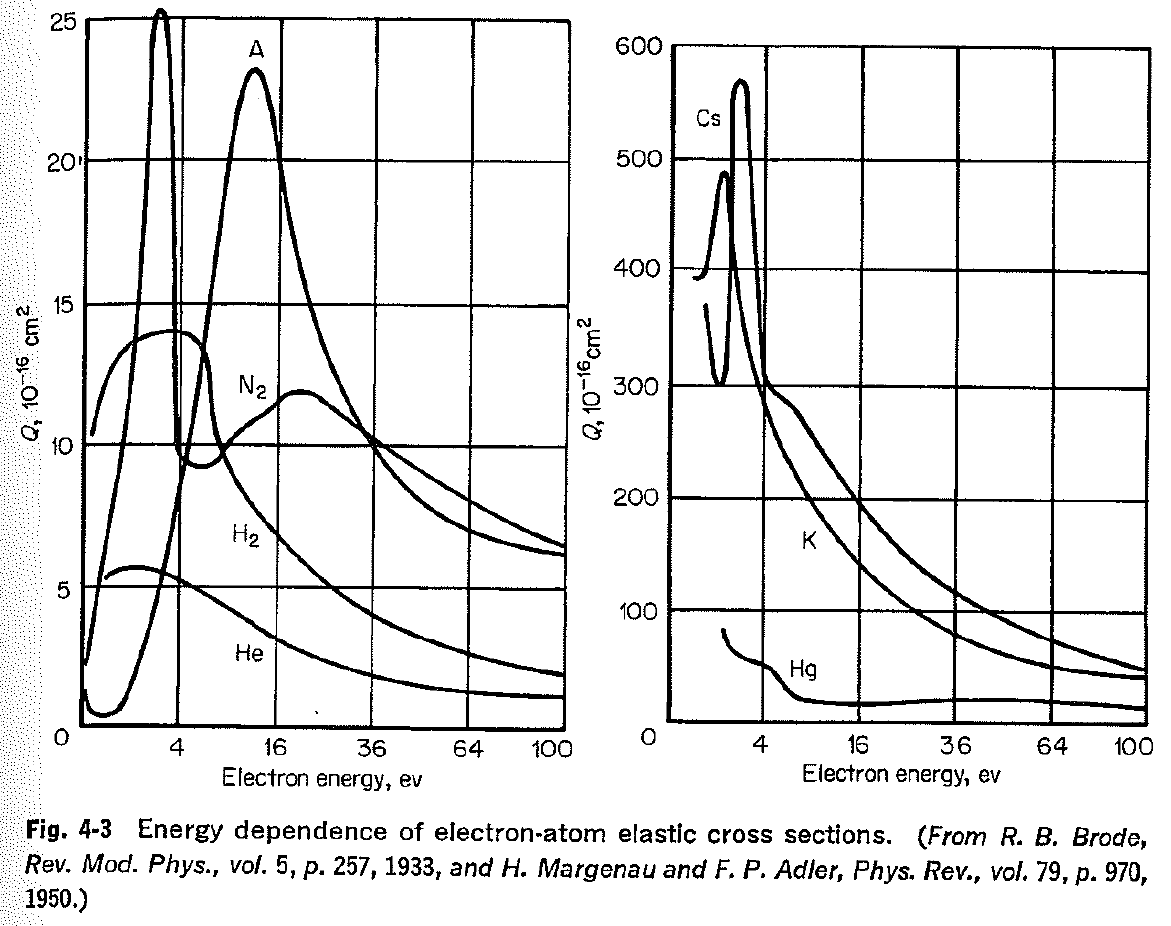
\includegraphics[scale=.45]{2.png}
\end{center}
\begin{center}
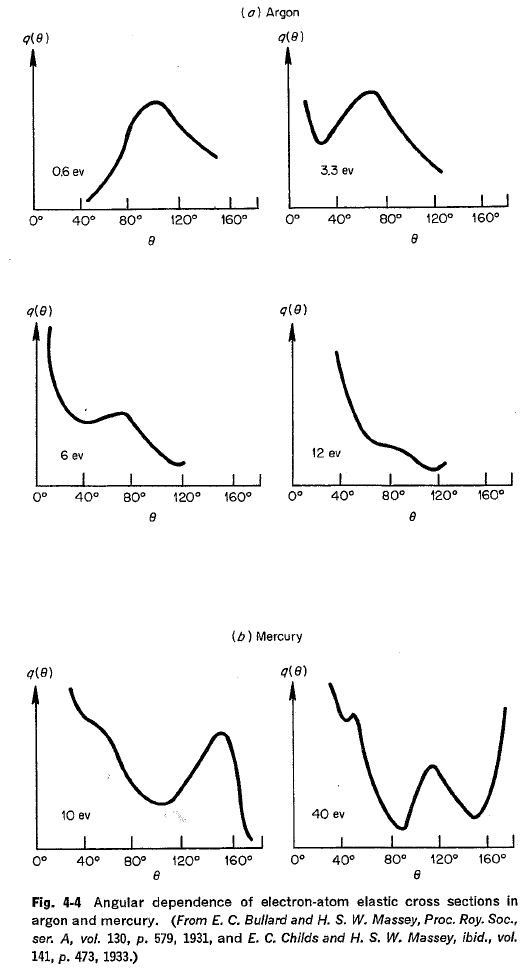
\includegraphics[scale=.45]{3.png}
\end{center}
\begin{center}
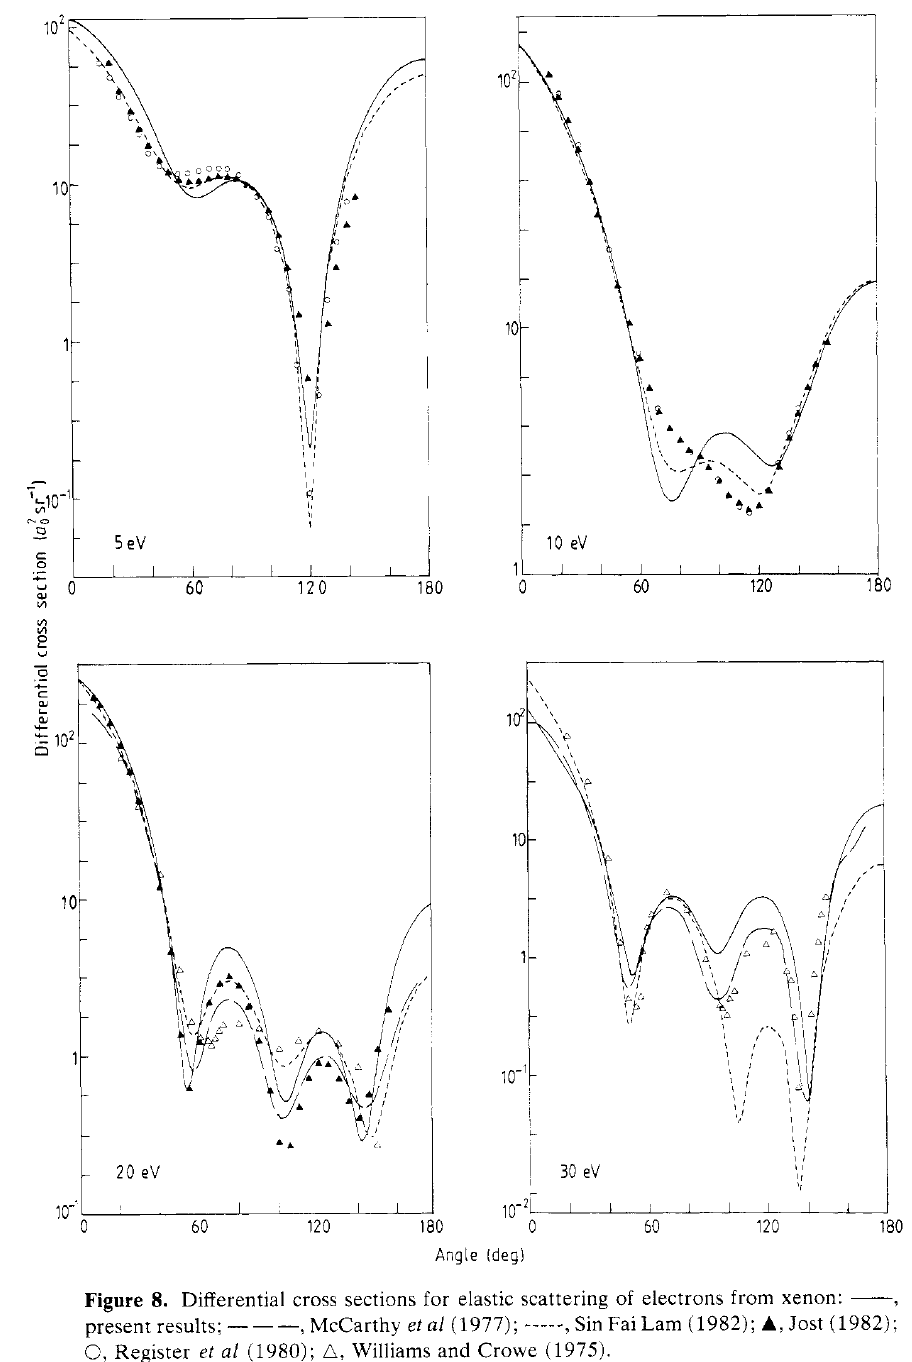
\includegraphics[scale=.45]{4.png}
\end{center}
\begin{center}
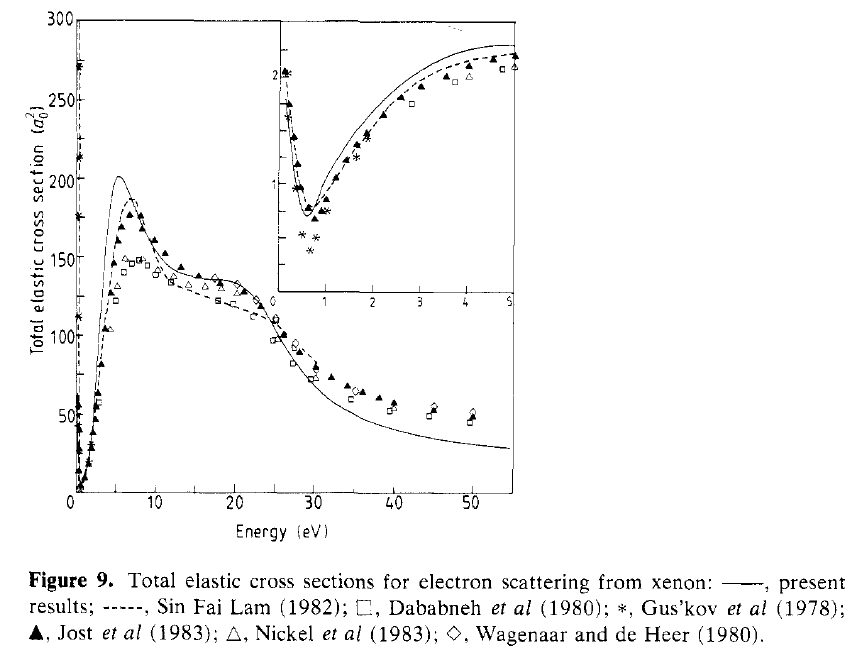
\includegraphics[scale=.45]{5.png}
\end{center}
Bohr radius squared (units)
\newpage
\subsection{Inelastic}
Most important reactions for EP.  Includes excitation (bound-bound transition)
 
 
And ionization (bound-free transition)
 
 
Both reactions require a certain threshold amount of energy, called the excitation potential           	or ionization potential          	.  In the above,
\begin{itemize}
   \item 	An electron with energy greater or equal to the excitation or ionization potential
   \item 	An excited atom (bound electron boosted to higher-energy orbit)
   \item 	An ion (bound electron ejected from valence shell)
 \end{itemize}
Typical excitation cross-sections for
\begin{center}
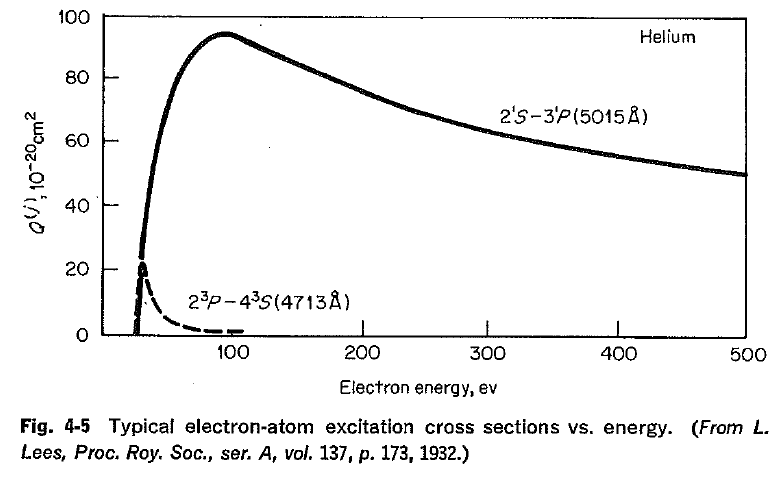
\includegraphics[scale=.45]{6.png}
\end{center}
 \begin{itemize}
\item "allowed" transition (by quantum mechanics rules) is the upper line; falls as 	
\item "forbidden" transition is lower line;  fall as
\end{itemize}
Note that cross-section drops to zero below                  	; simply conservation of energy (can't excite if impact energy is insufficient)
 
M Hayashi
Journal of Physics D: Applied Physics, Volume 16, Number 4
 
 \begin{center}
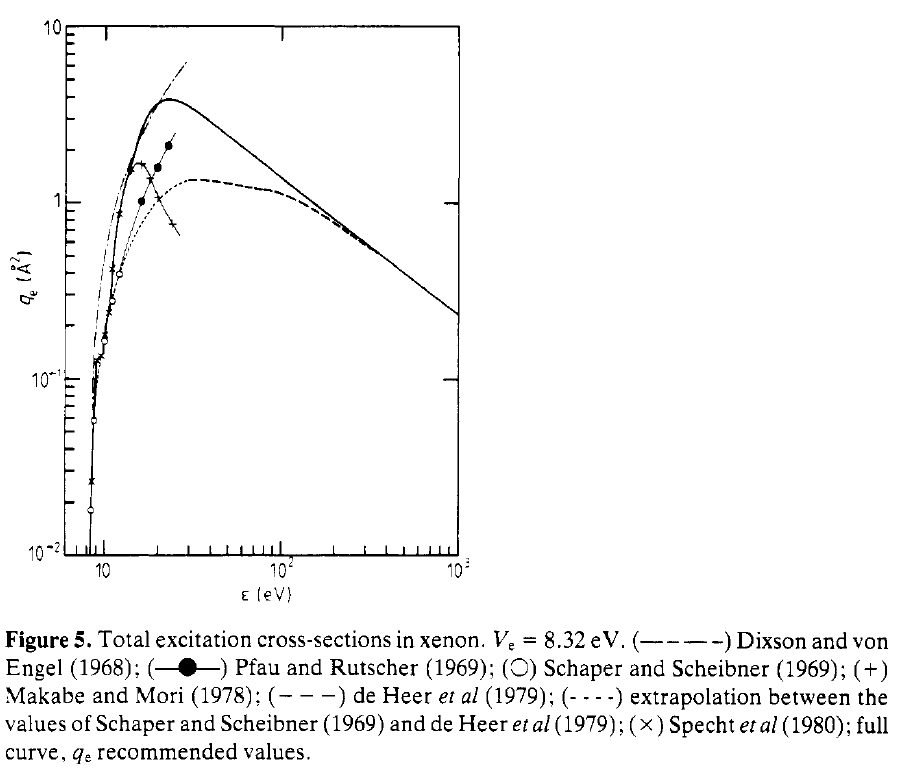
\includegraphics[scale=.45]{7.png}
\end{center}
 
Typical ionization cross-sections for
 
 \begin{center}
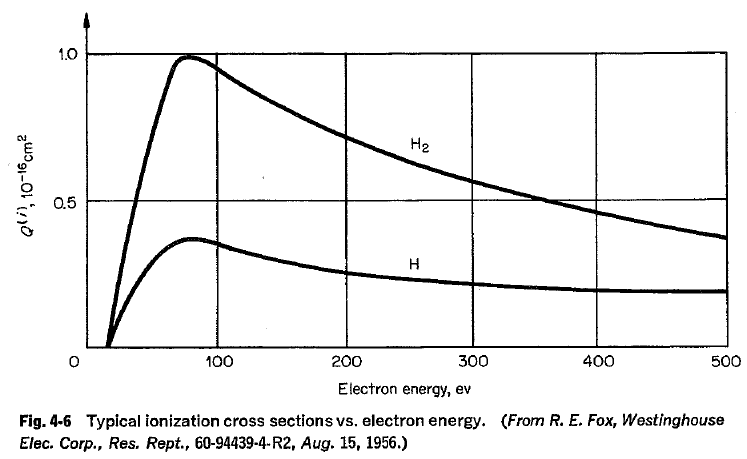
\includegraphics[scale=.45]{8.png}
\end{center}
 
  \begin{itemize}
\item Molecular hydrogen (upper line)
\item Atomic hydrogen (lower line)
 \end{itemize}
 \begin{center}
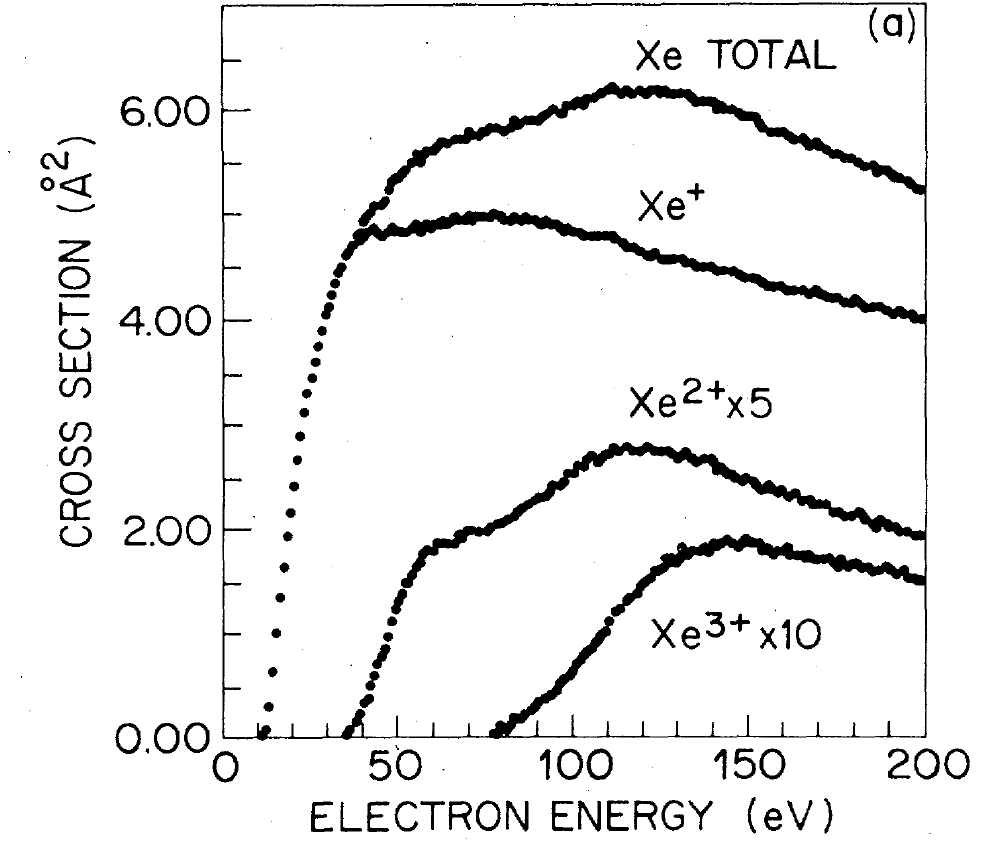
\includegraphics[scale=.45]{9.png}
\end{center}
Robert C. Wetzel, Frank A. Baiocchi, Todd R. Hayes, and Robert S. Freund
Phys. Rev. A 35, 559 ? Published 1 January 1987
 
 
 
Calculating the excitation and ionization rates:  mean electron speed is almost always much higher than mean neutral speed.
 
 
 
So the collision rate in a gas with number density na, is
 
 \begin{center}
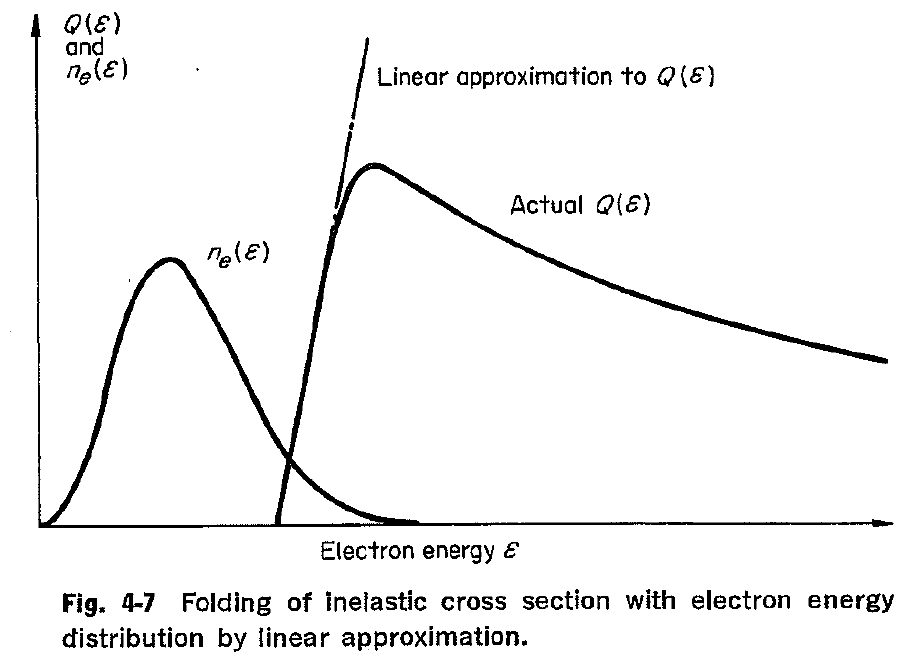
\includegraphics[scale=.45]{10.png}
\end{center}
 
Fig 4-7 shows
  \begin{itemize}
\item typical cross section Q
\item Electron energy distribution function,          (e.g., might be Maxwellian)
\item EEDF tails off around the peak of  Q , you can make a linear approximation in the collision rate integral (5.17)
\item Also note, only the high-energy tail of the EEDF participates in these processes (e.g., excitation, ionization)
\end{itemize}

\end{document}